\vspace*{4cm}
\part{Zigbee}\label{part:Zigbee}
Autor: Cyrill Horath
\vspace*{\fill}
\clearpage

\section{Einleitung}\label{sec:EinleitungZigbee}
In diesem Teil der Arbeit werden die Eigenschaften und Besonderheiten des Zigbee Mesh Stacks erläutert und es wird auf die Umsetzung des Benchmarks auf der Stack Ebene eingegangen. Es handelt sich um einen eigenständigen Teil in dem ausschliesslich der Zigbee Protokollstack behandelt wird.

\begin{wrapfigure}{r}{0.5\textwidth}
	\centering
	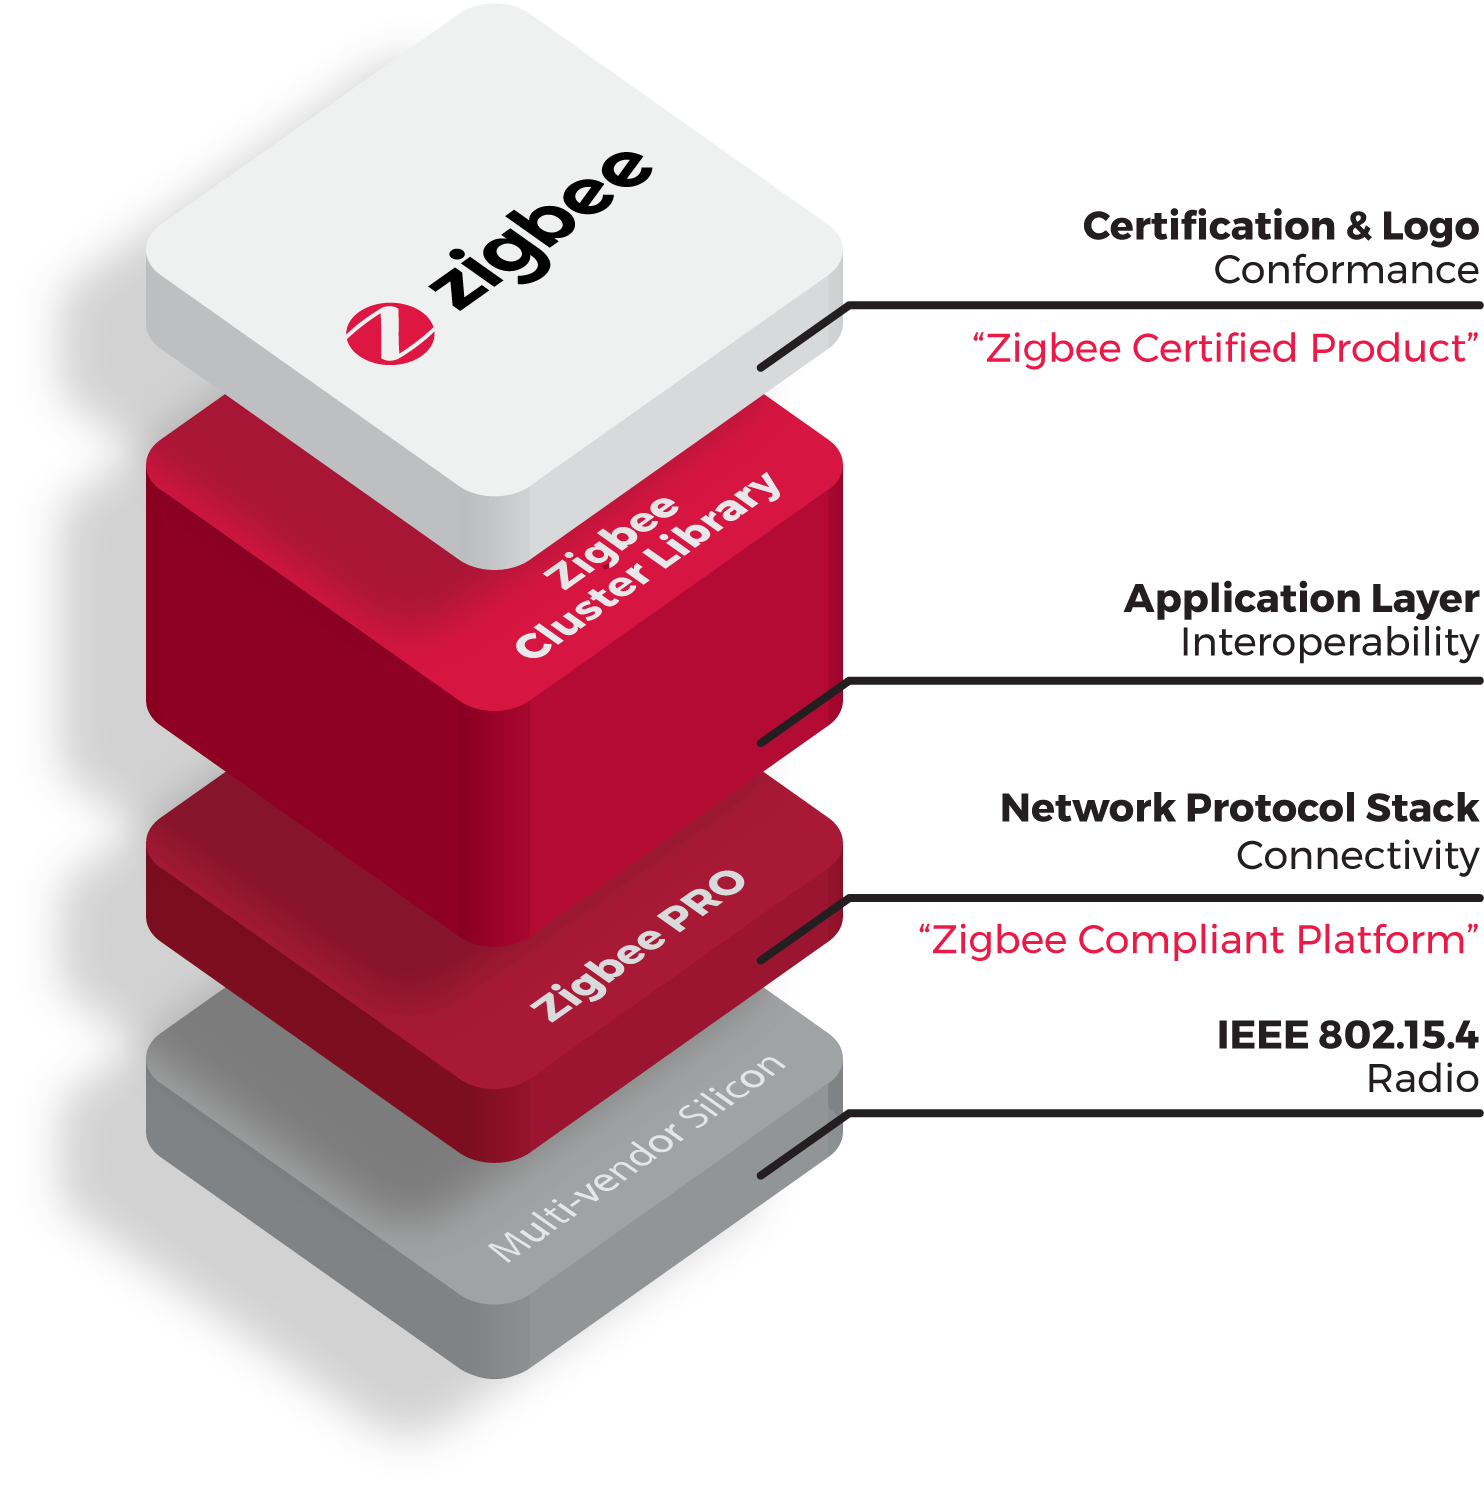
\includegraphics[width=0.5\textwidth]{Zigbee_Stack_symbolic.png}
	\caption{Zigbee Protokollstack}	\label{fig:ZigbeeProtokollstack}
\end{wrapfigure}

Zigbee ist ein auf dem \textit{IEEE 802.15.4} Standard aufbauendes, drahtloses Low Power Mesh Netzwerk Protokoll.
Es nutzt das im \textit{IEEE 802.15.4} Standard definierte ISM-Funkfrequenzband 2.4GHz und weitere Sub-GHz Bänder je nach Region und Bedarf.
Die im Jahre 2002 gegründete Zigbee Allianz ist Herausgeber der Zigbee Protokoll Spezifikation.
Unterdessen ist der Protokollstack bereits in der Version 3.0 spezifiziert.
Im Zuge der Verbreitung von Technologien in der Heim- Automatisierung erhielt auch Zigbee immer mehr Aufmerksamkeit und wuchs bis heute zudem am weitesten verbreiteten Mesh Netzwerk Protokoll in diesen Gebiet heran.
Besonders in Systemen für die Steuerung von Beleuchtungen wie zum Beispiel Phillips Hue oder Ikea Tradfri kommt Zigbee verbreitet zum Einsatz.

Die Spezifikationen innerhalb des Zigbee Protokollstacks sind weitreichend. Von der MAC Ebene über die Netzwerkschicht bis hin zur Applikationsebene gibt es klare Vorgaben, wie ein Zigbee Produkt aufgebaut sein soll (siehe Abbildung \ref{fig:ZigbeeProtokollstack}).
Mit der \textit{Zigbee Cluster Library} werden sogar spezifische Anwendungen vordefiniert wie beispielsweise die Steuerung einer Lichtquelle mit Dimmfunktion.
Diese Spezifikationen ermöglichen die Interoperabilität von Systemen mit der gleichen Funktion von unterschiedlichen Herstellern.